\documentclass[aspectratio=169]{beamer}
\usetheme{Madrid}
\usecolortheme{seahorse}
\setbeamertemplate{navigation symbols}{}

\usepackage{tikz}
\usetikzlibrary{positioning,arrows.meta,fit,shapes.geometric}

\begin{document}

\begin{frame}{Replication Status: Architecture, Scale, Limits, and Fixes}
\begin{columns}[T,totalwidth=\textwidth]
\begin{column}{0.55\textwidth}
\centering
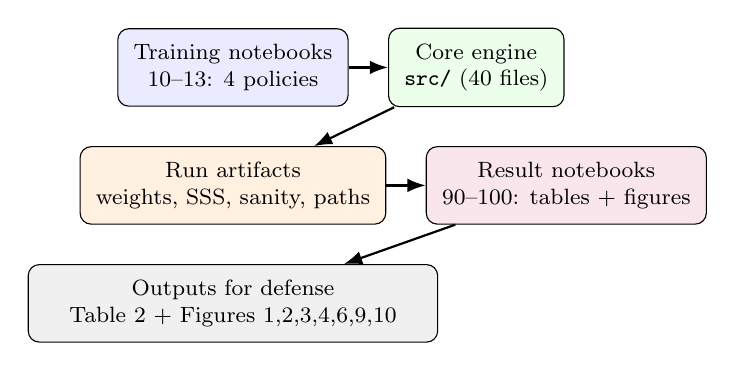
\begin{tikzpicture}[
  node distance=5mm and 5mm,
  box/.style={draw, rounded corners, align=center, font=\footnotesize, minimum height=8mm, inner sep=2mm},
  arr/.style={-Latex, thick}
]
  \node[box, fill=blue!8] (train) {Training notebooks\\10--13: 4 policies};
  \node[box, fill=green!8, right=of train] (core) {Core engine\\\texttt{src/} (40 files)};
  \node[box, fill=orange!12, below=of train] (art) {Run artifacts\\weights, SSS, sanity, paths};
  \node[box, fill=purple!10, right=of art] (res) {Result notebooks\\90--100: tables + figures};
  \node[box, fill=gray!12, below=of art, minimum width=52mm] (out) {Outputs for defense\\Table 2 + Figures 1,2,3,4,6,9,10};

  \draw[arr] (train) -- (core);
  \draw[arr] (core) -- (art);
  \draw[arr] (art) -- (res);
  \draw[arr] (res) -- (out);
\end{tikzpicture}
\end{column}

\begin{column}{0.45\textwidth}
\footnotesize
\textbf{Scale completed}
\begin{itemize}
  \item 4 trained policy pipelines: Taylor, modified Taylor, discretion, commitment.
  \item 14 notebooks, \textasciitilde 4.5k Python LOC in \texttt{src/}, \textasciitilde 2.0k code lines in notebooks.
  \item Full artifact chain saved per run: \texttt{weights.pt}, \texttt{weights\_best.pt}, SSS, sanity checks, \texttt{sim\_paths.npz}.
\end{itemize}

\textbf{Current limitations (honest)}
\begin{itemize}
  \item Strict sanity tolerances are not met on current MID runs (especially discretion/commitment).
  \item SSS and IRF levels for discretion/commitment still deviate from paper targets.
  \item Numerical burden is high for full-precision retraining on commitment branch.
\end{itemize}

\textbf{Fix path}
\begin{enumerate}
  \item Re-train discretion/commitment with stronger schedule and 3+ seeds.
  \item Accept runs only if sanity + residual gates pass before plotting.
  \item Rebuild Table 2 and all figures from selected validated runs only.
\end{enumerate}
\end{column}
\end{columns}
\vspace{0.3em}
\scriptsize \textit{Bottom line: the replication pipeline is complete end-to-end; the remaining gap is numerical quality control, not missing methodology blocks.}
\end{frame}

\end{document}
